\chapter{Requirements and Specifications} \label{ch:reqandspec}

As mentioned in section \ref{ch:introduction:sec:project_aims}, the overall goal of the project is to build a web application where teachers can create SQL assignments and students can submit solutions which are automatically graded. Therefore, the requirements of the project can be split in two parts: the requirements for the web application, and the requirements for the grading library, which can be implemented in a separate application. 

The library will be the main output of the project with the web application being just a basic interface for interacting with the library.

\section{Requirements} \label{ch:reqandspec:sec:rec}

\subsection{Web application}
\begin{enumerate}[label=R-\arabic*]
  \item The web application should be able to store data in a database;
  \item The web application should allow users to log in and keep their data
    across sessions;
  \item The web application should allow users to have different roles within the
    application (e.g. Student/ Teacher/ TA);
  \item  A teacher should be able to create assignments by giving a title, a description, and a SQL query that creates the tables and the relations between them, a SQL query that seeds the table with initial data, and a SQL query which represents the correct answer for the assignment;
  \item The application should compile the queries provided and, if no errors are shown, save the assignment in the database and display the schema of the database and the data from it;
  \item The teacher should be able to edit the assignments after they are created;
  \item The teacher should be able to delete assignments after they are created;
  \item A student should be able to provide solutions to assignments by submitting a SQL query. The web application should return the results instantly to the students after it assess the query. If any compilation errors are returned, they will be shown to the student;
  \item A student should be able to view the schema of the database for the assignment;
  \item A student should be able to see hints if they make any errors, or see a breakdown of the components from the teacher's query and the ones used by their query;
  \item SQL typing on the web application should be made in a browser-based code editor that provides syntax highlighting;
  \item Teachers should be able to have a graphical view of the results and download the results in a CSV format. In addition, they should be able to view the results of individual submissions.
\end{enumerate}

\subsection{Grading library}
\begin{enumerate}[label=G-\arabic*]
  \item The library should be able to connect to a \text{MySQL} server;
  \item The library should handle any error that might occur when communicating to the database (including failed execution of SQL queries, connection issues, etc.) and not throw away any unhandled errors;
  \item The library should provide a safe way to execute arbitrary queries that prevents any possible malicious actions (including SQL injection);
  \item The library should implement a grading algorithm for assessing SQL assignments; \label{req:grading}
  \item The library should provide a detailed explanation of the grade and how it was assessed; \label{req:grading_explanation}
  \item The library should provide hints about how a student could fix his query, if the query is wrong; \label{req:grading_hint}
  \item The library should expose a method that allows the compilation of an assignment given a schema query, a seed query, and a correct query. The application should return the schema and the data of the database if no errors are encountered. If errors are encountered, then it should return the appropriate error(s);
  \item The library should expose a method that allows the assessment of a submission given a schema query, a seed query, the instructor's correct query, and the submissions' query.  The assessment should be done with the grading algorithm implemented for requirement \ref{req:grading}. The result of the method should be the grade, the explanation implemented for \ref{req:grading_explanation}, and the hint returned from the implementation of \ref{req:grading_hint}.
\end{enumerate}

\section{Specifications} \label{ch:reqandspec:sec:spec}

These requirements can easily be implemented in a multitude of languages and frameworks as there are no language or framework-specific requirements. For this project, we have opted to build this in the Ruby programming language using two applications:
\begin{enumerate}
    \item A Ruby library (or gem, as it is called in Ruby) that will handle the requirements related to the grading of queries.
    \item A Ruby on Rails application that will handle the requirements related to the web application.
\end{enumerate}

The decision to split the application in two separate components was made in order to separate the concerns and to allow for independent work to happen on each application. Furthermore, by separating the library from the main web application we gain the ability to use the library in other cases (e.g. for building a Command-Line Interface). This also means that the library does not care about how the grades are displayed, or how the exercises and submissions are stored in the database.

Finally, by using a separate library, we can make use of encapsulation - hiding away the implementation details of grading from the web application, which is only meant to work with final results.

We have opted for a Ruby programming language based on the following criteria:

\begin{itemize}
    \item Past experience with the programming language and the associated framework means that more time could be spent on the grading algorithm, rather than learning a new language and a new framework.
    \item Ruby has database drivers for all popular databases. This means that, in the future, this application could be extended to run not only MySQL queries, but also other formats of queries. \footnote{While most queries use standard SQL, each database adds its own features which can make the queries incompatible with each other.}
    \item Ruby on Rails is one of the most popular and easy to use web application frameworks. It is a very opinionated framework, which means it took us less time deciding how to implement certain features.
\end{itemize}

\subsection{Development process} \label{ch:reqandspec:sec:spec:subsec:dev_process}

Although the two parts of the project allow parallel development, throughout the development of the project a waterfall approach will be used. The general pattern of development is the following:

\begin{enumerate}
  \item Implement and test feature in library and publish new version of the library;
  \item Update web application with the last version of library;
  \item Update the web application's existing code and test if any interfaces were changed;
  \item Implement and test new features in the web application.
\end{enumerate}

All the new features added in the library and the web application will be tested at the time of development. To ensure this, the following tools are used:
\begin{itemize}
  \item \textbf{Git \& Github Pull requests (PR)}: development will be done using the Git Version Control System. All new features will be developed on a separate branch than master, and to get them in master a new PR will be submitted on GitHub.
  \item \textbf{Travis} is a continuous integration system that will execute all tests from any Git commit. This will ensure that all features added are working according to the tests, and that existing features are not affected by the new changes.
  \item \textbf{Codecov} is a tool that calculates the code coverage of code from a PR. Whenever a new commit is pushed to a PR, Codecov's code coverage is recalculated and a message is left on the PR.
  \item \textbf{Rubocop} is a code linter that ensures the new code follows a standardized pattern (e.g. all strings use single quotes, not double quotes). While this tool does not test the code, by implementing code standards from the beginning we can ensure that they will be followed. Rubocop is executed on the CI step and is required for the CI to pass.
\end{itemize}
Both Travis and Codecov will provide \textit{checks} on Github PRs that are required for a PR to be merged.

\begin{figure}[htp]
    \centering
    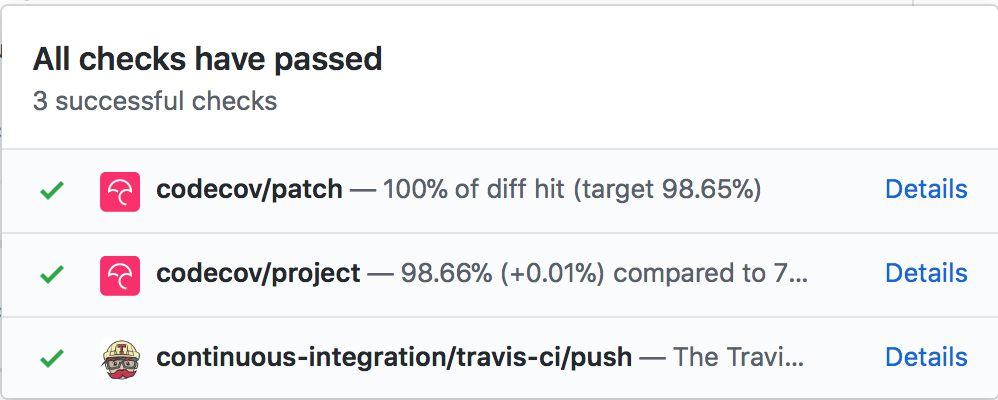
\includegraphics[width=(\linewidth / 3 * 2)]{Chapters/3-RequirementAndSpecifications/github_checks.png}
    \caption{GitHub PR checks}
    \label{fig:github_pr}
\end{figure}

\subsection{Platform requirements}

The application (including the library) has only two dependencies:
\begin{itemize}
  \item A MySQL server
  \item The ability to run Ruby (and Ruby on Rails)
\end{itemize}

\subsection{Specifications for the web application}

\begin{tabularx}{\textwidth}{|c|Y|Y|}
  \hline
  \textbf{R no.} & \textbf{Requirement details} & \textbf{Specification} \\\hline
  \endhead
  R-1 & The web application should be able to store data in a database & Use Ruby on Rails' ActiveRecord to store and access data in a MySQL server \\\hline
  R-2 & The web application should allow users to log in and keep their data across sessions. & Use the devise library for authentication and provide sign-in and sign-up functionality using devise\\\hline
  R-3 &  The web application should allow users to have different roles within the application (e.g.Student/ Teacher/ TA) & Use pundit library for user roles management and authorization\\\hline
  R-4 &  A teacher should be able to create assignments by giving a title, a description, and a SQL query that creates the tables and the relations between them, a SQL query that seeds the table with initial data, and a SQL query which represents the correct answer for the assignment. & Provide a web form built where teachers can create new assignments. The form will be built using Bootstrap, and the code editors should use codemirror to provide code syntax highlighting. \\\hline
  R-5 &  The application should compile the queries provided and, if no errors are shown, save the assignment in the database and display the schema of the database and the data from it. & Use the compile method provide by the library and defined and display any error that may occur, otherwise save the record in the database. \\\hline
  R-6 & The teacher should be able to edit the assignments after they are created. & Recompile the query and update the assignment in the database, if no errors are encountered. \\\hline
  R-7 & The teacher should be able to delete assignments after they are created. & Deletes the challenge from database \\\hline
  R-8 & A student should be able to provide solutions to assignments by submitting a SQL query. The web application should return the results instantly to the students after it assess the query. If any compilation errors are returned, they will be shown to the student. & Provide a web form built in Bootstrap that provides a code editor using codemirror. Assess the query using the assess method provided by the grading library. Save all submissions in the database after they have been assessed. \\\hline
  R-9 & A student should be able to view the schema of the database for the assignment. & Render a HTML view that contains the schema of the database and provides a form written in Bootstrap and codemirror where they provide solutions. \\\hline
  R-10 & A  student  should  be  able  to  see  hints  if  they make any  errors, or see a breakdown of the components from the teacher’s query and the ones used by their query. & Display a HTML view based on the results of their submission, after being graded. \\\hline
  R-11 & SQL typing on the web application should be made in a browser-based code editor that provides syntax highlighting. & Provide a code editor written in codemirror. \\\hline
  R-12 & Teachers should be able to have a graphical view of the results and download the results in  a CSV format.   In  addition,  they  should  be  able  to  view  the  results  of individual submissions. & Provide a download CSV button that gets the best submission of each student for a certain assignment. Provide a HTML view that displays the result of a individual submission. \\\hline
\end{tabularx}

\subsection{Specification for the grading library}

\begin{tabularx}{\textwidth}{|c|Y|Y|}
  \hline
  \textbf{R no.} & \textbf{Requirement details} & \textbf{Specification} \\\hline
  \endhead
G-1 & The library should be able to connect to a MySQL server. & Connect to a MySQL database using Ruby library mysql2. \\\hline
G-2 & The library should handle any error that might occur when communicating to the database (including failed execution of SQL queries, connection issues, etc.) and not throw away any unhandled errors. & Handle errors returned by mysql2 and return library-specific errors. \\\hline
G-3 & The library should provide a safe way to execute arbitrary queries that prevents any possible malicious actions (including SQL injection). & Execute the queries in a separate database using a user that has restricted permissions. \\\hline
G-4 & The library should implement a grading algorithm for assessing SQL assignments. & Implement a grading algorithm that follows the grading algorithm defined by XData. This means the grading will compare the components of two canonicalized queries. Therefore, the algorithm will contain two components: the canonicalization of a SQL query and the comparison of components. \\\hline
G-5 & The library should provide a detailed explanation of the grade and how it was assessed. & Return a grade for each component and the components after they have been canonicalized. \\\hline
G-6 & The library should provide hints about how a student could fix his query, if the query is wrong & Return the most relevant hint for the query. The relevance of the hint will be determined by two factors: the grade of the component, and a predefined importance ordering of components\\\hline
G-7 & The library should expose a method that allows the compilation of an assignment given a schema query, a seed query, and a correct query. The application should return the schema and the data of the database if no errors are encountered. If errors are encountered, then it should return the appropriate error(s). & Execute the queries and handle any errors if they occur and return them as mentioned in specifications for G-1 and G-2. Extract the tables created in the schema query and then extract the data inserted in the seed query. \\\hline
G-8 & The library should expose a method that allows the assessment of a submissions given a schema query, a seed query, the instructor's correct query, and the submissions' query.  The assessment should be done with the grading algorithm implemented for requirement \ref{req:grading}. The result of the method should be the grade, the explanation implemented for \ref{req:grading_explanation} and the hint returned from the implementation of \ref{req:grading_hint}. & Execute the queries, handle any errors if they occur, and return them as mentioned in specifications for G-1 and G-2. Apply the grading algorithm implemented for G-4 and return the grade, the detailed breakdown of the grade implemented for G-5 and the hint from G-6. \\\hline
\end{tabularx}
